\documentclass[t, pdftex]{beamer}
\usetheme[]{Cockrell}
%\usetheme[dept=Aerospace\ Engineering\ and\ Engineering\ Mechanics]{cockrell}
%\usetheme[dept=Biomedical\ Engineering]{cockrell}
%\usetheme[dept=Chemical\ Engineering]{cockrell}
%\usetheme[dept=Civil,\ Architectural\ and\ Environmental\ Engineering]{cockrell}
%\usetheme[dept=Electrical\ and\ Computer\ Engineering]{cockrell}
%\usetheme[dept=Mechanical\ Engineering]{cockrell}
%\usetheme[dept=Materials\ Science\ and\ Engineering]{cockrell}
%\usetheme[dept=Petroleum\ and\ Geosystems\ Engineering]{cockrell}

% Packages
%\usepackage{etex}
%\usepackage[bigfiles]{media9}
%\graphicspath{{./figs/}}

%Enable cancelto in math
\usepackage{cancel}
\usepackage[]{algorithm2e}
\usepackage{mathtools}
\usepackage{pgfgantt}
\usepackage[version=3]{mhchem} % Package for chemical equation typesetting \ce{}
\usepackage{siunitx} % Provides the \SI{}{} and \si{}
\renewcommand{\CancelColor}{\color{utorange}}

%Add bibliography file location for citiation
\bibliography{example.bib}


\title{A Hi2Low Method for Improving\\ CRUD Predictions}
\subtitle{}
\author{William Gurecky}
\institute{UT Austin Mechanical Engineering}
\date{\today}


\begin{document}

% =========================================================================== %
\titleframe
\frame{\frametitle{Outline}\tableofcontents}

% =========================================================================== %
\begin{frame}[shrink=10]
    \frametitle{Chalk River Unidentified Deposit (CRUD)}
    CRUD forms a porous layer on the surface of fuel rods.
    \begin{itemize}
    \item Preferentially deposited where temperature is high - near or above saturation point - and where local shear stresses on the rod are low.
	\item CRUD induced local corrosion (CILC).
    \item CRUD induced power shift (CIPS). In industry known as axial offset anomaly (AOA).
    \begin{itemize} 
    	\item CRUD and tends to uptake and retain boron from the coolant.
    	\item \ce{Li^+} + \ce{B(OH)_3}   $\rightarrow$ \ce{LiBO_2} + \ce{H^+} + \ce{H_2O} .
    \end{itemize}
    \item CASL developed CRUD simulation packages: MAMBA \& Mongoose
    \end{itemize}
%\begin{figure}[!htbp]
%\centering
%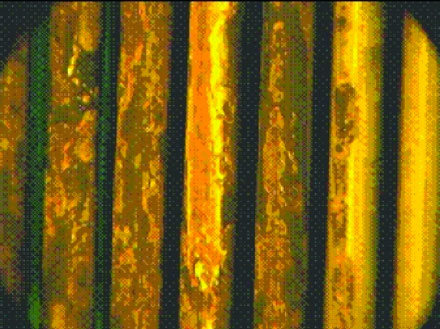
\includegraphics[width=4cm]{figs/crud-crud.jpg}
%\caption{CRUD on fuel rods.}
%\label{log_closed}
%\end{figure}
%
    \begin{figure}
        \centering
        \begin{minipage}{.7\textwidth}
            \centering
            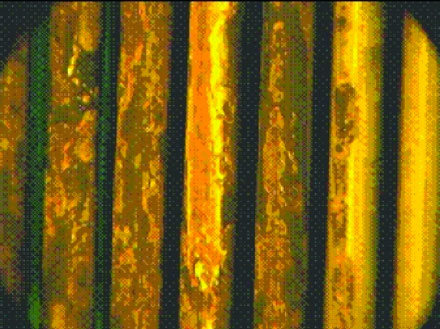
\includegraphics[width=6cm]{figs/crud-crud.jpg}
        \end{minipage}%
        \begin{minipage}{.4\textwidth}
            \centering
            \includegraphics[width=6cm]{figs/crud_flake_ex.png}
        \end{minipage}
    \end{figure}
\end{frame}

% =========================================================================== %
\section{Background}
\begin{frame}
    \frametitle{Chalk River Unidentified Deposit (CRUD)}
    \begin{figure}
        \centering
        \begin{minipage}{.5\textwidth}
            \centering
            \includegraphics[width=6cm]{figs/ao_mpact_ctf.png}
            \caption{Core averaged \% axial offset. [CASL-I-2015-0318-000]}
        \end{minipage}%
        \begin{minipage}{.5\textwidth}
            \centering
            \includegraphics[width=6cm]{figs/core_b10_mpact_ctf.png}
            \caption{VERA WBNP1 Cycle 7 CRUD \ce{^{10}B}. 16.08 $[MWD/MTU]$}
        \end{minipage}
    \end{figure}
\end{frame}

% =========================================================================== %
\begin{frame}[shrink=20]
    \frametitle{Coupled CFD/CRUD Calculation}
    \begin{itemize}
    \item CFD/CRUD coupling is useful for single-pin or single-assembly CRUD estimates.
    \item High fidelity CFD/CRUD simulations are too numerically costly for full core simulation.
    \end{itemize}
        \begin{figure}[!htbp]
\centering
\includegraphics[width=14cm]{figs/combo_180x.png}
\label{log_closed}
    \end{figure}
\end{frame}

% =========================================================================== %
\begin{frame}
Differences between CTF (subchannel) and CFD meshes for a single pin.
\begin{figure}
        \centering
        \begin{minipage}{.4\textwidth}
            \centering
            \includegraphics[width=3cm]{figs/cfd_ctf_mesh_v.png}
        \end{minipage}%
        \begin{minipage}{.4\textwidth}
            \centering
            \includegraphics[width=2cm]{figs/ctf_mesh_v.png}
        \end{minipage}
\end{figure}
\end{frame}

% =========================================================================== %
\section{Hi2Low Approach}
\begin{frame}
    \frametitle{CFD informed surrogate model to improve CRUD growth}
    \begin{itemize}
    \item Construct a scale bridging model which utilizes a suite of pre-computed CFD solutions to improve CRUD predictions given on the CTF grid. 
    \item CTF estimates mean TH conditions everywhere in the core at a low spatial resolution.  The surrogate provides higher order moments about the mean.
    \end{itemize}
    \begin{block}{Rod Surface Field}
        \[ 
        F(\mathbf z) = \underbrace{\mu(\mathbf{z})}_\text{CTF} + \underbrace{\varepsilon({\mathbf z, \mathbf p(\mathbf z)})}_\text{CFD Informed} + b(\mathbf{z})
        \]
    \end{block}
    Treat $\varepsilon$ as a random field.  $\varepsilon(\cdot)$ is a CFD informed model. $\mathbf z$ are spatial coordinates. $\mathbf p$ are a set of auxiliary predictors. \\
    $b$ is bias ($\mu_{CTF} - \mu_{CFD}$) \\
    $\mu$ are spatially averaged over a CTF patch
\end{frame}

% =========================================================================== %
\begin{frame}\frametitle{Objectives}
\begin{itemize}
\item Account for fine scale flow features unresolved by CTF on the growth of CRUD and boron hideout.
\item Proposed Hi2Low Approach:
\begin{itemize}
	\item Forgo attempting to capture spatial distributions of temperature, boundary heat flux and TKE on rod surface. 
	\item Instead, track joint probability density $f(T, TKE, q'')$ tallied over coarse CTF patches.
\end{itemize}
	\item Predict likelihood of temperatures in excess of saturation occurring in coincidence with low local turbulent kinetic energy.
	\item Preserve correlations between surface temperature, boundary heat flux and turbulent kinetic energy.
\end{itemize}
\end{frame}

% =========================================================================== %
\begin{frame}[shrink=10]
    \frametitle{Prior Art: HTC Remapping Hi2Low Procedure}
\begin{columns}
\begin{column}{0.5\textwidth}
   \begin{itemize}
   \item Salko et. al (2017) developed a Hi2Low procedure based on mapping and re-scaling CFD results onto an intermediate reconstruction grid upon which CRUD is grown.
   \item The single phase heat transfer coefficient (HTC) and TKE surface fields are mapped.
   \item An iterative method is used to converge on the correct pin surface temperature given HTC and the boundary heat flux provided by CTF.
   \end{itemize}
\end{column}
\begin{column}{0.5\textwidth}  %%<--- here
    \begin{center}
    \begin{figure}
     \includegraphics[width=5cm]{figs/cfd_ctf_multi_grid.png}
     \caption{TKE remapping procedure.}      
    \end{figure}
     \end{center}
\end{column}
\end{columns}
\end{frame}

% =========================================================================== %
\begin{frame}
    \frametitle{Prior Art: HTC Remapping Hi2Low Procedure}
    \begin{figure}[!htbp]
\centering
\begin{minipage}{.5\textwidth}
  %
  \includegraphics[width=5cm]{figs/ctf_crud_orig.png}
\caption{CRUD growth on the rod surface prior to HTC and TKE field remapping.}
\label{fig:crud_pre_map}
\end{minipage}%
\begin{minipage}{.5\textwidth}
  %
  \includegraphics[width=5cm]{figs/ctf_crud_reconstructed.png}
\caption{CRUD growth on the rod surface post HTC and TKE field remapping.}
\label{fig:crud_post_map}
\end{minipage}
\end{figure}
\end{frame}


% =========================================================================== %
\begin{frame}
\begin{figure}[!htbp]
\centering
\includegraphics[width=10.88cm]{figs/ctf_patch_ex3.png}
\label{model_overview}
\end{figure}
\end{frame}

% =========================================================================== %
\begin{frame}
On a single coarse CTF patch:
\begin{figure}[!htbp]
\centering
\includegraphics[width=11cm]{figs/model_relations.png}
\label{model_overview}
\end{figure}
\end{frame}

% =========================================================================== %
\section{Capturing Dependence between Random Variables}
\begin{frame}
\frametitle{Capturing Dependence - Sklar's Theorem}
\begin{itemize}
\item Given joint CDF: $H$, w/ cumulative margins: $F(x)=P[X < x] = \int_{-\infty}^{x}f(t)dt$
\[
H(x,y) = C(F(x), F(y))
\]
\[
c(u, v) = \frac{\partial^2 C(u, v)}{\partial u \partial v};\ u=F(x), v=F(y)
\]
\item  The copula PDF, $c(\cdot)$ is describes dependence between two random variables.
\item  Has uniform marginal density distributions \cite{Nelsen2006}.
\item  Defined on the unit square $[0, 1]^2$ (in the bivariate case)
\item  Any joint PDF, $h(\cdot)$ can be decomposed as: \\
\[
h(x, y) = c(F(x), F(y)|\theta_c)f(x|\theta_x)f(y|\theta_y)
\]
Where $\theta_c$ and $\theta_{x,y}$ are free copula and marginal model parameters respectively.
\end{itemize}
\end{frame}


% =========================================================================== %
\begin{frame}
\frametitle{Specifying Copula Parameters}
\begin{itemize}
\item For the case of Archimedean copula, Kendall's tau, $\rho_\tau$ is
related to the copula's shape parameter by:
\[
\rho_\tau = 1 + 4 \int_0^1 \frac{\varphi(\theta_c,t)}{\varphi'(\theta_c, t)}dt
\]
Where $\varphi(\theta_c, t)$ is the copula's generator function and $\varphi'$ is the first derivative of the generator function with respect to $t$.
\item  If we restrict ourselves to the class of  Archimedean copula we only need $\rho_\tau$ and the copula type, $\Theta_c$ (gumbel, frank, clayton, ect.) to approximately specify the dependence structure between the temperature and turbulent kinetic energy residual distributions in each CTF patch.
\item Must associate each CTF patch with a copula family (categorical response) and Kendall's tau (real-valued).
\end{itemize}
\end{frame}

% =========================================================================== %
\begin{frame}
\frametitle{Non-Parametric Representation of the Margins}
\begin{figure}[!htbp]
\centering
\includegraphics[width=7cm,angle=90,origin=c]{figs/scanned_cdf.pdf}
\label{model_overview}
\end{figure}

\end{frame}

% =========================================================================== %
\begin{frame}
\frametitle{Single CRUD Step on a CTF Patch}
The $i^{th}$ CRUD sample drawn from CTF patch, $j$:
\begin{figure}[!htbp]
\centering
\includegraphics[width=9cm]{figs/crud_samples.png}
\label{model_overview}
\end{figure}
\begin{itemize}
\item Samples are drawn with weight $w_i=A_p/N$ where $A_p$ is the CTF patch area and $N$ is the total number of samples/patch.
\item TH boundary conditions are held fixed throughout the duration of the CRUD simulation step with timestep size $\Delta t$.
\end{itemize}
\end{frame}

% =========================================================================== %
\begin{frame}
\tiny Single CRUD Step on a CTF Patch: Example Results $@$ 100 [days] simulation time
\begin{figure}[!htbp]
\centering
\includegraphics[width=8cm]{figs/new/patch_scatter.png}
\label{model_overview}
\end{figure}
\end{frame}

% =========================================================================== %
\begin{frame}
\frametitle{Time Stepping: Reordering samples on a CTF Patch}
Two bounding cases to consider:
\begin{itemize}
\item Assume: Hot spots on the rod surface remain stationary w.r.t time
	\begin{itemize}
	\item Re-order samples such that the highest temperature sample always occures in the same location inside a patch.
	\end{itemize}
\item Converse: Hot spots randomly move about the rod as time goes on
	\begin{itemize}
	\item Randomize samples inside a patch - do not preserve any spatial structure of the temperature distribution.
	\end{itemize}
\end{itemize}
Define a metric $\alpha T_i + \beta TKE_i + \gamma q_i'' = m_i$. Rank $m_i's$ by highest to lowest with and store the ranked indicies.  Use sorted indicies to re-order the samples on the patch.
\end{frame}

% =========================================================================== %
\begin{frame}
\frametitle{Time Stepping: Comparing Approaches}
    \begin{figure}
        \centering
        \begin{minipage}{.5\textwidth}
            \centering
            \includegraphics[width=6cm]{figs/new/patch_rand_t_ex.png}
            \caption{Randomized temperature samples on a patch.}
        \end{minipage}%
        \begin{minipage}{.5\textwidth}
            \centering
            \includegraphics[width=6cm]{figs/new/patch_t_ex.png}
            \caption{Re-ordered temperature samples}
        \end{minipage}
    \end{figure}
Both patches share the \emph{same} PDF of Temperture, however, the spatial distibutions are not equal.
\end{frame}

% =========================================================================== %
\begin{frame}
\frametitle{Time Stepping: Comparing Approaches}
    \begin{figure}
        \centering
        \begin{minipage}{.5\textwidth}
            \centering
            \includegraphics[width=6cm]{figs/new/patch_rand_tke_ex.png}
            \caption{Randomized TKE samples on a patch.}
        \end{minipage}%
        \begin{minipage}{.5\textwidth}
            \centering
            \includegraphics[width=6cm]{figs/new/patch_tke_ex.png}
            \caption{Re-ordered TKE samples}
        \end{minipage}
    \end{figure}
Both patches share the \emph{same} PDF of TKE, however, the spatial distibutions are not equal.
\end{frame}

% =========================================================================== %
\begin{frame}
\frametitle{Time Stepping: Single Pin Results}
\tiny{Pin-integrated Boron inside the CRUD as a function of time.  Green: Assumes randomly moving hot spots.  Blue: Assumes stationary hot spots.}
\begin{figure}[!htbp]
\centering
\includegraphics[width=8cm]{figs/new/cmpr_pin_totals.png}
\label{model_overview}
\end{figure}
\end{frame}


% =========================================================================== %
\section{Results}
\begin{frame}
\frametitle{Single Pin Results $@$ 100 days}
    \begin{figure}
        \centering
        \begin{minipage}{.5\textwidth}
            \centering
            \includegraphics[width=6cm]{figs/new/struct_pin_z_twall.png}
            \caption{Outiside Clad Temp $[K]$.}
        \end{minipage}%
        \begin{minipage}{.5\textwidth}
            \centering
            \includegraphics[width=6cm]{figs/new/struct_pin_z_bmass.png}
            \caption{ Boron Linear Deposition $[g/cm]$}
        \end{minipage}
    \end{figure}
\end{frame}


\lastframe%

\end{document}
